
\documentclass[12pt,a4paper]{article}
\usepackage[T1]{fontenc}
\usepackage[utf8]{inputenc}

\usepackage{lmodern,amsmath,amssymb,mathtools,bm,booktabs,tabularx,array,multirow}
\usepackage[margin=20mm,top=19mm,bottom=19mm,headheight=15pt,headsep=6mm,footskip=8mm]{geometry}
\usepackage{graphicx,caption,subcaption,float,xcolor,titlesec,fancyhdr,hyperref,microtype,enumitem}
\usepackage{siunitx}
\definecolor{aghgreen}{HTML}{006E53}\definecolor{aghred}{HTML}{B32A38}\definecolor{ink}{HTML}{253242}
\hypersetup{colorlinks=true,urlcolor=aghgreen,linkcolor=aghgreen,citecolor=aghgreen,pdfauthor={Hamzeh Khanpour},pdftitle={Higgs Physics at the FCC mu+ e- Collider -- 20-page Research Note}}
\titleformat{\section}{\large\bfseries\color{aghgreen}}{\thesection}{0.65em}{}
\titleformat{\subsection}{\normalsize\bfseries\color{ink}}{\thesubsection}{0.6em}{}
\titlespacing*{\section}{0pt}{0.7ex}{0.65ex}
\titlespacing*{\subsection}{0pt}{0.65ex}{0.4ex}
\captionsetup{font=small,labelfont=bf,skip=3pt}
\setlength{\parindent}{0pt}\setlength{\parskip}{6.3pt}\linespread{1.18}
\setlist[itemize]{noitemsep,topsep=3pt,leftmargin=1.5em}
\pagestyle{fancy}\fancyhf{}\fancyhead[L]{\footnotesize\color{aghgreen}\textbf{FCC-$\mu^+e^-$ Higgs physics}}\fancyhead[R]{\footnotesize Internal research note $\cdot$ November 2026}
\fancyfoot[L]{\footnotesize AGH University of Krakow $\vert$ Preliminary LO phenomenology}\fancyfoot[R]{\footnotesize\thepage/20}
\renewcommand{\headrulewidth}{0.3pt}\renewcommand{\footrulewidth}{0pt}
\newcommand{\newnote}{\clearpage}
\newcommand{\smallsource}[1]{\par\vspace{-2pt}{\footnotesize\color{gray}\raggedright\emph{Source/status: #1}\par}}
\newcommand{\eps}{\varepsilon}
\newcommand{\Lumi}{\mathcal{L}}
\newcommand{\sig}{\sigma}
\newcommand{\kth}{\kappa_3}
\newcommand{\ktwo}{\kappa_{2V}}
\newcommand{\hh}{hh}
\newcommand{\CC}{\mathrm{CC}}
\newcommand{\NC}{\mathrm{NC}}
\newcommand{\lo}{\mathrm{LO}}


\begin{document}
% PAGE 1

\begin{center}
{\color{aghgreen}\rule{\linewidth}{2pt}}\\[6pt]
{\LARGE\bfseries Higgs Physics at the FCC-$\boldsymbol{\mu^+e^-}$ Collider}\\[6pt]
{\large\bfseries Production Mechanisms, Polarization, Self-Couplings, and a Collaborative Research Roadmap}\\[8pt]
{\normalsize A scientific handout for the first FCC-$\mu^+e^-$ Higgs-physics collaboration meeting}\\[5pt]
{\bfseries Hamzeh Khanpour}\\
AGH University of Krakow, Faculty of Physics and Applied Computer Science\\
\emph{Discussion participants:} Hamzeh Khanpour, Krzysztof Piotrzkowski, Richard Ruiz, Piotr Kotko\\
November 2026\\[5pt]
{\color{aghred}\rule{0.4\linewidth}{1pt}}
\end{center}


\textbf{Abstract.}\; A polarized high-energy antimuon--electron collider could combine the cleanliness of lepton initial states with multi-TeV electroweak fusion and a distinct experimental complement to FCC-ee. This note reviews the Higgs physics case of the proposed FCC-$\mu e$ facility, develops the underlying electroweak amplitudes, and reconciles the available leading-order MadGraph calculations. The completed inclusive campaign comprises four Standard Model final states---charged-current (CC) and neutral-current (NC) single- and double-Higgs production---evaluated at exact centre-of-mass energies of 1 and 2 TeV for six positive-muon polarizations. All 48 configurations were produced with an unpolarized electron beam and stable Higgs bosons. The charged-current rates follow the expected $1+P_{\mu^+}$ enhancement; neutral-current rates rise more weakly, with slopes near 0.22. The strong relative energy growth of $hh$ production motivates direct investigations of the Higgs trilinear self-interaction and $hhVV$ gauge vertices. Earlier $hh\to4b$, complete four-bottom, associated-$b\bar b h$, and muon-collider $Zh$ calculations are reviewed with their distinct cuts and normalization conventions. The genuine MadGraph Feynman diagrams confirm inclusion of the $h^*\to hh$ self-coupling, separate Higgs emissions, and $hhVV$ contact contributions. A physically consistent strategy is proposed for coupling scans, differential measurements, realistic signal/background likelihoods and an exploratory triple-Higgs feasibility test. No anomalous-coupling limits or triple-Higgs cross sections are claimed as completed results.

\textbf{Key message.} The existing LO results form a benchmark and consistency test, \emph{not} a detector-level estimate of coupling precision. The next scientific deliverable is a common, validated $hh$ theory-and-analysis framework for combining CC, NC, polarization and differential information.

%\smallsource{Internal CERN MadGraph calculations (preliminary); collider concept: Piotrzkowski, arXiv:2610.40451v2 \cite{piotr}; underlying numerical provenance in the accompanying CSV and audit.}



% PAGE 2
\newnote

\section{The proposed FCC-$\mu e$ facility: kinematics and operating points}
For ultrarelativistic head-on beams of energies $E_e$ and $E_\mu$, conservation of four-momentum gives
\begin{equation}
 s=(p_e+p_\mu)^2\simeq4E_eE_\mu,\qquad \sqrt{s}\simeq 2\sqrt{E_eE_\mu}.
 \label{eq:s}
\end{equation}
Unlike symmetric $e^+e^-$ beams, the highly asymmetric configuration has a boosted centre-of-mass frame. If $+z$ is defined along the incoming antimuon, its rapidity is approximately
\begin{equation}
 y_{\rm CM}=\frac12\ln\frac{E_{\mu^+}}{E_{e^-}};
 \quad \text{at }(2000,120)\,{\rm GeV},\quad y_{\rm CM}\simeq1.41.
\end{equation}
Consequently, a central Higgs system in the CM frame may be forward in the laboratory. Acceptance and detector geometry cannot be inferred from an inclusive cross section alone.



\begin{table}[H]\centering\small
\caption{Two deliberately distinct energy families. The earlier points are approximate FCC-$\mu e$ machine benchmarks; the later ones are the exact-energy numerical scan.}
\begin{tabular}{@{}llll@{}}\toprule
Study & $E_{\mu^+}$ & $E_{e^-}$ & $\sqrt{s}$\\\midrule
Earlier design-like & 2 TeV & 120 GeV & 0.9798 TeV\\
Earlier design-like & 5 TeV & 183 GeV & 1.9131 TeV\\
Inclusive CERN scan & 2 TeV & 125 GeV & 1.0000 TeV\\
Inclusive CERN scan & 5 TeV & 200 GeV & 2.0000 TeV\\\bottomrule
\end{tabular}\end{table}
Piotrzkowski's revised proposal \cite{piotr} explores a facility based on ultracold $\mu^+$ generation, acceleration and a storage ring, potentially operated with FCC-ee infrastructure. It is a \emph{proposed} machine concept, not an operating collider. The main scientific motivation is access to weak-boson fusion at energies above the traditional Higgsstrahlung regime, without a hadronic beam remnant. The antimuon decay chain also motivates a potentially high-intensity neutrino programme.

The proposal should not be described using a single universal luminosity. Its v2 Table~1 reports two 2-TeV-antimuon working points: $\sqrt{s}=0.60$ TeV with instantaneous luminosity $4.5\times10^{34}$ and $\sqrt{s}=0.98$ TeV with $0.63\times10^{34}\,{\rm cm}^{-2}{\rm s}^{-1}$. A previous version quoted a different 0.98-TeV example. These are model-dependent performance assumptions, not guaranteed delivered datasets; $\mathrm{ab}^{-1}$ projections require live time, availability and luminosity integration.
\smallsource{FCC-$\mu e$ proposal v2, especially Secs. 2--4 and Table 1 \cite{piotr}; energies computed with Eq.~\eqref{eq:s}.}




% PAGE 3
\newnote

\section{Why complement FCC-ee? Higgs opportunities and experimental constraints}
FCC-ee's precision programme emphasizes well-controlled $e^+e^-$ reactions, especially $e^+e^-\to Zh$ around 240 GeV, precise Higgs decay and width information, and complementary measurements near 365 GeV. The FCC Feasibility Study \cite{fcc} discusses these as prospective capabilities with explicit luminosity and detector assumptions. The proposed FCC-$\mu e$ does not replace that programme: it probes a different collision regime, including multi-TeV spacelike $W$ and $Z$ exchange, and offers direct tree-level access to $hh$ amplitudes that contain the Higgs trilinear coupling.

%\begin{figure}[H]\centering
%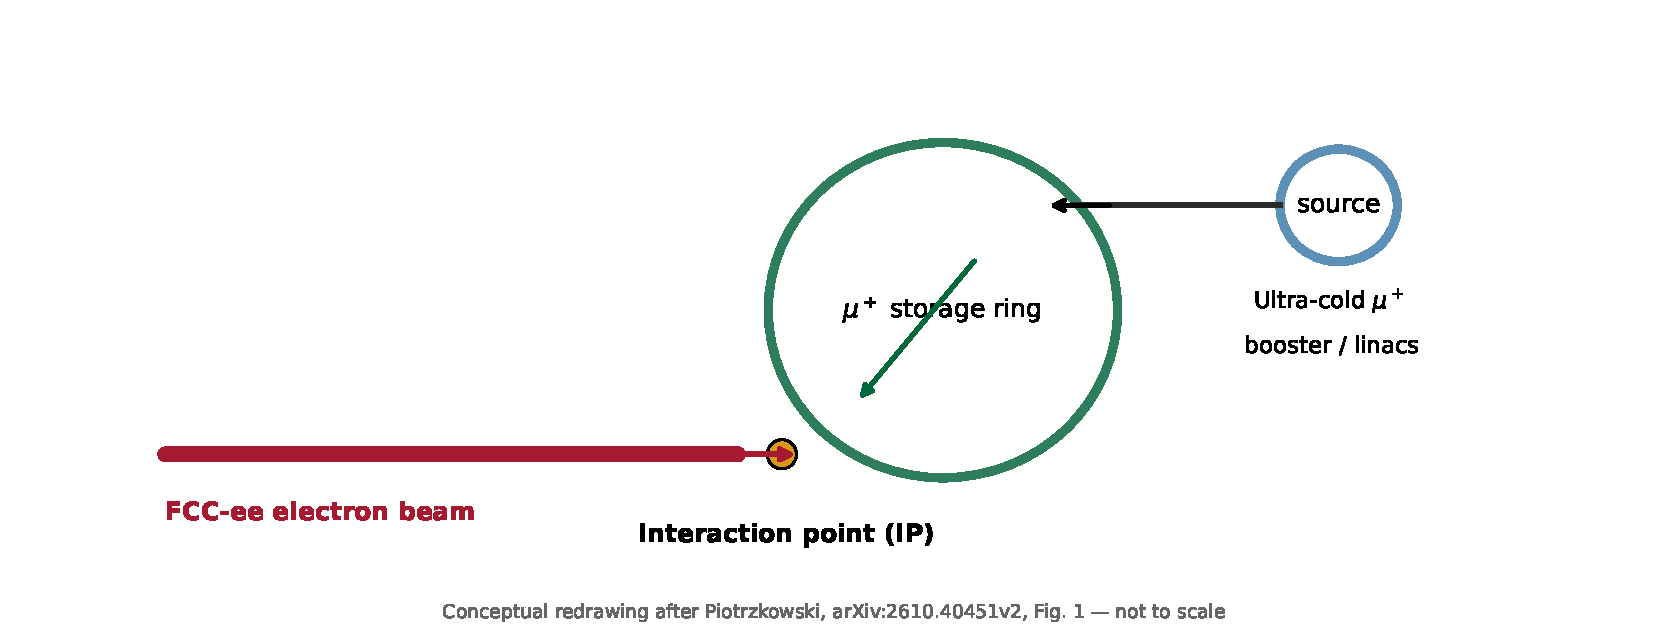
\includegraphics[width=0.93\linewidth,height=0.29\textheight,keepaspectratio]{figures/Figure_FCCmue_concept_schematic.pdf}
%\caption{Redrawn conceptual schematic, \emph{not to scale}, based on the FCC-$\mu e$ proposal; not the original figure from \cite{piotr}.}
%\end{figure}

In $\mu^+e^-$ collisions the incoming lepton flavours differ; ordinary flavour-conserving $s$-channel annihilation of an $e^+e^-$ or $\mu^+\mu^-$ pair is absent. This changes associated-production backgrounds, but it does not make the physics background-free. For CC fusion, neutrinos carry away longitudinal and transverse momentum. For NC fusion, the scattered electron and antimuon can be very forward, making their acceptance and beam-pipe backgrounds decisive.

Crucial feasibility issues include antimuon source intensity and emittance preservation, muon-decay-induced electromagnetic backgrounds, shielding/nozzle geometry, beam-beam interactions, detector vertex coverage, event reconstruction under substantial boosts, and realistic polarized integrated luminosities. The proposed collision programme therefore requires close integration of Higgs phenomenology with machine and detector parameterizations. Sensitivities must eventually be shown as a function of $\sqrt{s}$, luminosity, beam polarization, forward instrumentation and selection efficiency, not simply inferred by scaling cross sections from another collider.

\textbf{Complementarity hypothesis:} FCC-ee can constrain input $hVV$ couplings and Higgs branching fractions; FCC-$\mu e$ can add polarization-tagged CC/NC $h$ and $hh$ fusion information, potentially resolving self-coupling and contact-interaction degeneracies in a combined fit. This is a research programme to test, not an already established quantitative improvement.



% PAGE 4
\newnote

\section{Electroweak symmetry breaking and normalized Higgs interactions}
The Higgs field is an $SU(2)_L$ doublet of hypercharge $Y=1/2$. In unitary gauge its vacuum configuration can be written as $\Phi=(0,(v+h)/\sqrt2)^T$. The renormalizable scalar and gauge-kinetic Lagrangian contains
\begin{align}
\mathcal L_\Phi&=(D_\mu\Phi)^\dagger(D^\mu\Phi)-V(\Phi),\\
V(\Phi)&=-\mu^2\Phi^\dagger\Phi+\lambda(\Phi^\dagger\Phi)^2,
\qquad v^2=\mu^2/\lambda.
\end{align}
Substituting $\Phi$ and eliminating the tadpole at the minimum, $m_h^2=2\lambda v^2$, yields the physical scalar potential, up to an irrelevant additive constant,
\begin{equation}\label{eq:potential}
V(h)=\frac12m_h^2h^2+\frac{m_h^2}{2v}h^3+\frac{m_h^2}{8v^2}h^4.
\end{equation}
With the explicit convention $\mathcal L\supset -\lambda_3h^3/3!-\lambda_4h^4/4!$, the Standard Model values are $\lambda_3^{\rm SM}=3m_h^2/v$ and $\lambda_4^{\rm SM}=3m_h^2/v^2$. The associated Feynman rules are $-i\lambda_3$ and $-i\lambda_4$. Using these conventions matters: some references instead call the coefficients in $V(h)$ ``the couplings,'' differing by factorials.

The gauge-boson mass terms obtained from $|D_\mu\Phi|^2$ also fix the one- and two-Higgs interactions:
\begin{equation}\label{eq:gaugeh}
\mathcal L\supset m_W^2W_\mu^+W^{-\mu}\left(1+\frac{2h}{v}+\frac{h^2}{v^2}\right)
+\frac12m_Z^2Z_\mu Z^\mu\left(1+\frac{2h}{v}+\frac{h^2}{v^2}\right).
\end{equation}
Taking functional derivatives yields $hWW:\ 2im_W^2g_{\mu\nu}/v$ and $hhWW:\ 2im_W^2g_{\mu\nu}/v^2$, with the analogous $Z$ rules after the identical-field factors are included. At tree level, these couplings are correlated by the doublet structure; independent effective modifications require a declared parameterization.

For the physics programme it is useful to introduce $\kappa_W$, $\kappa_Z$, $\kappa_{2W}$, $\kappa_{2Z}$, $\kappa_3$ and $\kappa_4$ as ratios of corresponding vertices to the SM values. A universal $\kappa_{2V}$ is a shorthand only if the selected theory links the $hhWW$ and $hhZZ$ shifts. The single-Higgs channels primarily test $hVV$ at tree level; double Higgs combines $hVV$, $hhVV$ and the self-interaction.




% PAGE 5
\newnote

\section{Weak-boson fusion, helicity, interference, and unitarity}
The dominant Higgs-production mechanism of interest is the exchange of spacelike electroweak bosons from the incoming charged leptons. A schematic factorized expression is
\begin{equation}
\mathrm d\sigma(\mu^+e^-\to X+h^{(n)})\sim
\sum_{V_1V_2,\lambda_1\lambda_2}
 f_{V_1/\mu^+}^{\lambda_1}\otimes f_{V_2/e^-}^{\lambda_2}
 \otimes\mathrm d\hat\sigma(V_1V_2\to h^{(n)}),
\end{equation}
where $n=1,2,3$. This effective-vector-boson language is valuable for interpreting the high-energy behaviour, but is not a replacement for the full gauge-consistent $2\to3,4,5$ matrix element. The bosons are typically off shell, the exact final-state kinematics matter, and interference among physical tree graphs must be retained.

For longitudinal weak bosons, the Goldstone-boson equivalence theorem exposes the cancellations implied by symmetry breaking. In a common nonlinear Higgs effective description,
\begin{equation}
\frac{v^2}{4}{\rm Tr}\!\left[(D_\mu U)^\dagger D^\mu U\right]
\left(1+2a\frac{h}{v}+b\frac{h^2}{v^2}+\cdots\right),
\end{equation}
the energy-growing term in $V_LV_L\to hh$ is, up to overall phase and sign conventions, proportional to $(b-a^2)s/v^2$. It cancels at leading power in the SM ($a=b=1$). A departure between $hhVV$ and $(hVV)^2$ modifies this cancellation and may enhance the high-$m_{hh}$ tail. This motivates simultaneous control of $\kappa_V$ and $\kappa_{2V}$ rather than interpreting a total $hh$ cross section only in terms of $\kappa_3$.

The off-shell self-coupling contribution contains a scalar propagator $(m_{hh}^2-m_h^2)^{-1}$ and is often relatively influential closer to the $hh$ threshold. However, no individual graph defines a separately measurable ``self-coupling cross section.'' Schematically,
\begin{equation}
\sigma_{hh}\propto\int\mathrm d\Phi\,
\left|\mathcal M_{hhVV}+\mathcal M_{\mathrm{separate}}+\mathcal M_{h^*\to hh}\right|^2.
\end{equation}
The squares and cross terms may differ greatly over phase space. Only a complete amplitude, or an explicitly valid gauge-invariant operator expansion, is a robust basis for a parameter fit. This distinction is central to Krzysztof's original diagram question and to the collaboration's future anomalous-coupling scan.




% PAGE 6
\newnote

\section{Charged-current single Higgs: $\mu^+e^-\to\bar\nu_\mu\nu_e h$}
The charged-current (CC) single-Higgs process is generated by the complete LO Standard Model command
\begin{center}\ttfamily\small generate e- mu+ > ve vm\textasciitilde{} h QCD=0\end{center}
The two incoming charged leptons radiate weak charged currents, which fuse through the $hWW$ vertex. At the amplitude level the process tests the $SU(2)_L$ structure of the weak current together with the $hWW$ coupling. It is therefore the natural high-statistics calibration channel for subsequent CC double-Higgs studies. It does not contain a tree-level $h^*\to hh$ self-coupling contribution, and a single inclusive rate alone cannot disentangle $hWW$ strength from luminosity, polarization or decay normalization.

For negligible lepton masses, an electron charged current selects a left-handed electron and a positive antimuon of right helicity. Let $P_{e^-}=(N_R-N_L)/(N_R+N_L)$ for electrons and analogously $P_{\mu^+}$ for antimuons. With helicity fractions $(1-P_{e^-})/2$ and $(1+P_{\mu^+})/2$, and only one CC initial-helicity combination contributing at leading power,
\begin{equation}\label{eq:ccpol}
\sigma_{\CC}(P_{e^-},P_{\mu^+})\simeq
(1-P_{e^-})(1+P_{\mu^+})\,\sigma_{\CC}(0,0).
\end{equation}
This counts relative to the unpolarized average. With the actual study's $P_{e^-}=0$, the enhancement is $R_{\CC}=1+p$, where $p=P_{\mu^+}/100$.

The completed exact-energy simulation gives $\sigma_{\CC h}(0)=210.540\pm0.209$ fb at 1 TeV and $386.010\pm0.303$ fb at 2 TeV. At +80\% polarization these become $378.570\pm0.243$ and $695.000\pm0.614$ fb. The corresponding normalized rate enhancements of approximately 1.8 provide a clear check of beam-polarization implementation. Errors quoted here are Monte Carlo integration uncertainties only. A practical $hWW$ determination would exploit several Higgs decay channels with controlled efficiencies and backgrounds, fit the acceptance-corrected rate, and combine FCC-ee or other inputs to break branching-ratio and total-width degeneracies.

The immediate differential observables are Higgs transverse momentum and rapidity, missing transverse momentum, and angular correlations with reconstructed Higgs decays. Their laboratory distributions are strongly influenced by the asymmetric beam boost, meaning that $\eta$ acceptance and momentum coverage must be included before inferring sensitivity.




% PAGE 7
\newnote

\section{Neutral-current single Higgs: $\mu^+e^-\to\mu^+e^-h$}
The complete NC process uses
\begin{center}\ttfamily\small generate e- mu+ > e- mu+ h QCD=0\end{center}
and contains the tree-level neutral weak-boson fusion amplitude. Both outgoing charged leptons can populate small scattering angles. Even when the total inclusive weak-fusion rate is finite, an experimentally useful prediction requires realistic acceptance, beam-pipe masking, and stability scans in the forward region. A numerical ``no-cuts'' result is not automatically a detector fiducial prediction.

At high energy, both left- and right-chiral charged leptons couple to $Z$, with dimensionless coefficients (stripping the common $g/c_W$ factor)
\begin{equation}
 g_L=-\tfrac12+s_W^2,\qquad g_R=s_W^2,
 \qquad s_W^2\equiv\sin^2\theta_W.
\end{equation}
If the neutral-boson-fusion amplitude has approximately the same kinematic weighting for the corresponding positive-muon helicities, the inclusive polarization ratio is
\begin{equation}\label{eq:ncpol}
R_{\NC}(p)\simeq1+A_{\NC}p,\quad
A_{\NC}\simeq\frac{g_L^2-g_R^2}{g_L^2+g_R^2}.
\end{equation}
The antimuon helicity convention interchanges the particle-chirality language, so the sign of $A_{\NC}$ should always be defined with the beam convention explicitly. Equation~\eqref{eq:ncpol} is a leading pure-$Z$ approximation: exact full-process predictions depend on the electroweak input scheme and any subleading amplitudes. The MG5 parameter card should be consulted before assigning a specific numerical weak mixing angle.

The CERN results give $\sigma_{\NC h}(0)=20.835\pm0.025$ fb at 1 TeV and $38.991\pm0.030$ fb at 2 TeV. At +80\% antimuon polarization, the results are $24.476\pm0.015$ and $45.829\pm0.055$ fb, respectively. Thus the NC enhancement is about 17.5%, much smaller than the CC value of roughly 80%. The NC single-H rate is approximately one tenth of CC single H at these energies.

Experimentally, the final-state electron and antimuon may permit useful event classification, but only if both can be tagged with credible angular and energy coverage. A differential NC analysis should keep $p_T^{e,\mu}$, $\eta_{e,\mu}$ and momentum-transfer distributions, not merely $\sigma(\NC h)$. Combining this with CC data offers a complementary test of $hZZ/hWW$ interactions and their electroweak correlations.




% PAGE 8
\newnote

\section{Double-Higgs production: physics content and coupling dependence}
For charged-current and neutral-current channels the unrestricted MG5 processes are, respectively,
\begin{center}\ttfamily\small
 generate e- mu+ > ve vm\textasciitilde{} h h QCD=0\\
 generate e- mu+ > e- mu+ h h QCD=0
\end{center}
The Higgs-pair amplitude contains three structurally distinct tree-level mechanisms: a direct $hhVV$ contact interaction, diagrams with Higgs bosons emitted through separate $hVV$ vertices and an intermediate off-shell scalar with $V^*V^*\to h^*\to hh$. The third mechanism depends on the trilinear coupling $\lambda_3$. Neither the contact topology nor the separately emitted Higgs topology may be removed while retaining a claim to the \emph{full} SM cross section.

With $\kappa_W,\kappa_Z$ denoting single-Higgs gauge coupling modifiers and $\kappa_{2W},\kappa_{2Z}$ the relevant contact modifiers, a phenomenological amplitude may be schematically organized as
\begin{equation}\label{eq:hhamp}
\mathcal M_{hh}=\kappa_{2V}\mathcal M_c^{\rm SM}
+\kappa_V^2\mathcal M_t^{\rm SM}
+\kappa_V\kappa_3\mathcal M_s^{\rm SM},
\end{equation}
with $V=W$ for CC and $V=Z$ for NC, and with a definition of the modified theory required to make the decomposition precise. For fixed other parameters, $\sigma_{hh}(\kappa_3)=c_0+c_1\kappa_3+c_2\kappa_3^2$. The coefficient $c_1$ is a physically important interference term and can be negative. A total-rate measurement may admit two distinct $\kappa_3$ solutions; the $m_{hh}$ distribution and correlated channels can help resolve this ambiguity.

The SM inclusive unpolarized CC double-Higgs rate grows from $0.0743838\pm0.0001274$ fb at exact 1 TeV to $0.418510\pm0.0006568$ fb at 2 TeV, a factor $5.63$. For NC double H the corresponding rates are $0.00962012\pm0.0000146$ and $0.0547116\pm0.0000851$ fb, a factor $5.69$. This is substantially larger relative energy growth than for single H, consistent with increased multi-particle phase space and vector-boson luminosities.

Nevertheless, $\kappa_3$ has \emph{not} yet been scanned in these 48 SM runs. The existing physics potential is a motivation and a design input for such a study, not a realized coupling constraint. The central research objective is to identify which combination of rate, threshold spectrum and polarization is robust against correlated $hVV$ and $hhVV$ modifications.



% PAGE 9
\newnote

\section{Original CERN Feynman diagrams: an explicit amplitude check}
Krzysztof asked whether the calculations include both $h^*\to hh$ through the trilinear self-interaction and the diagrams in which the two Higgs bosons couple separately to weak bosons. The original process exports answer this directly. Each of the two $hh$ processes contains four tree-level diagrams, as labeled in the original MadGraph files: diagram 1 is the $hhWW$ or $hhZZ$ contact term, diagrams 2 and 3 are separate $hVV$ emission topologies, and diagram 4 contains the off-shell scalar $h^*\to hh$. All four contribute coherently to the original generator-level cross sections.


\begin{figure}[H]
\centering
\begin{subfigure}[t]{0.48\linewidth}\centering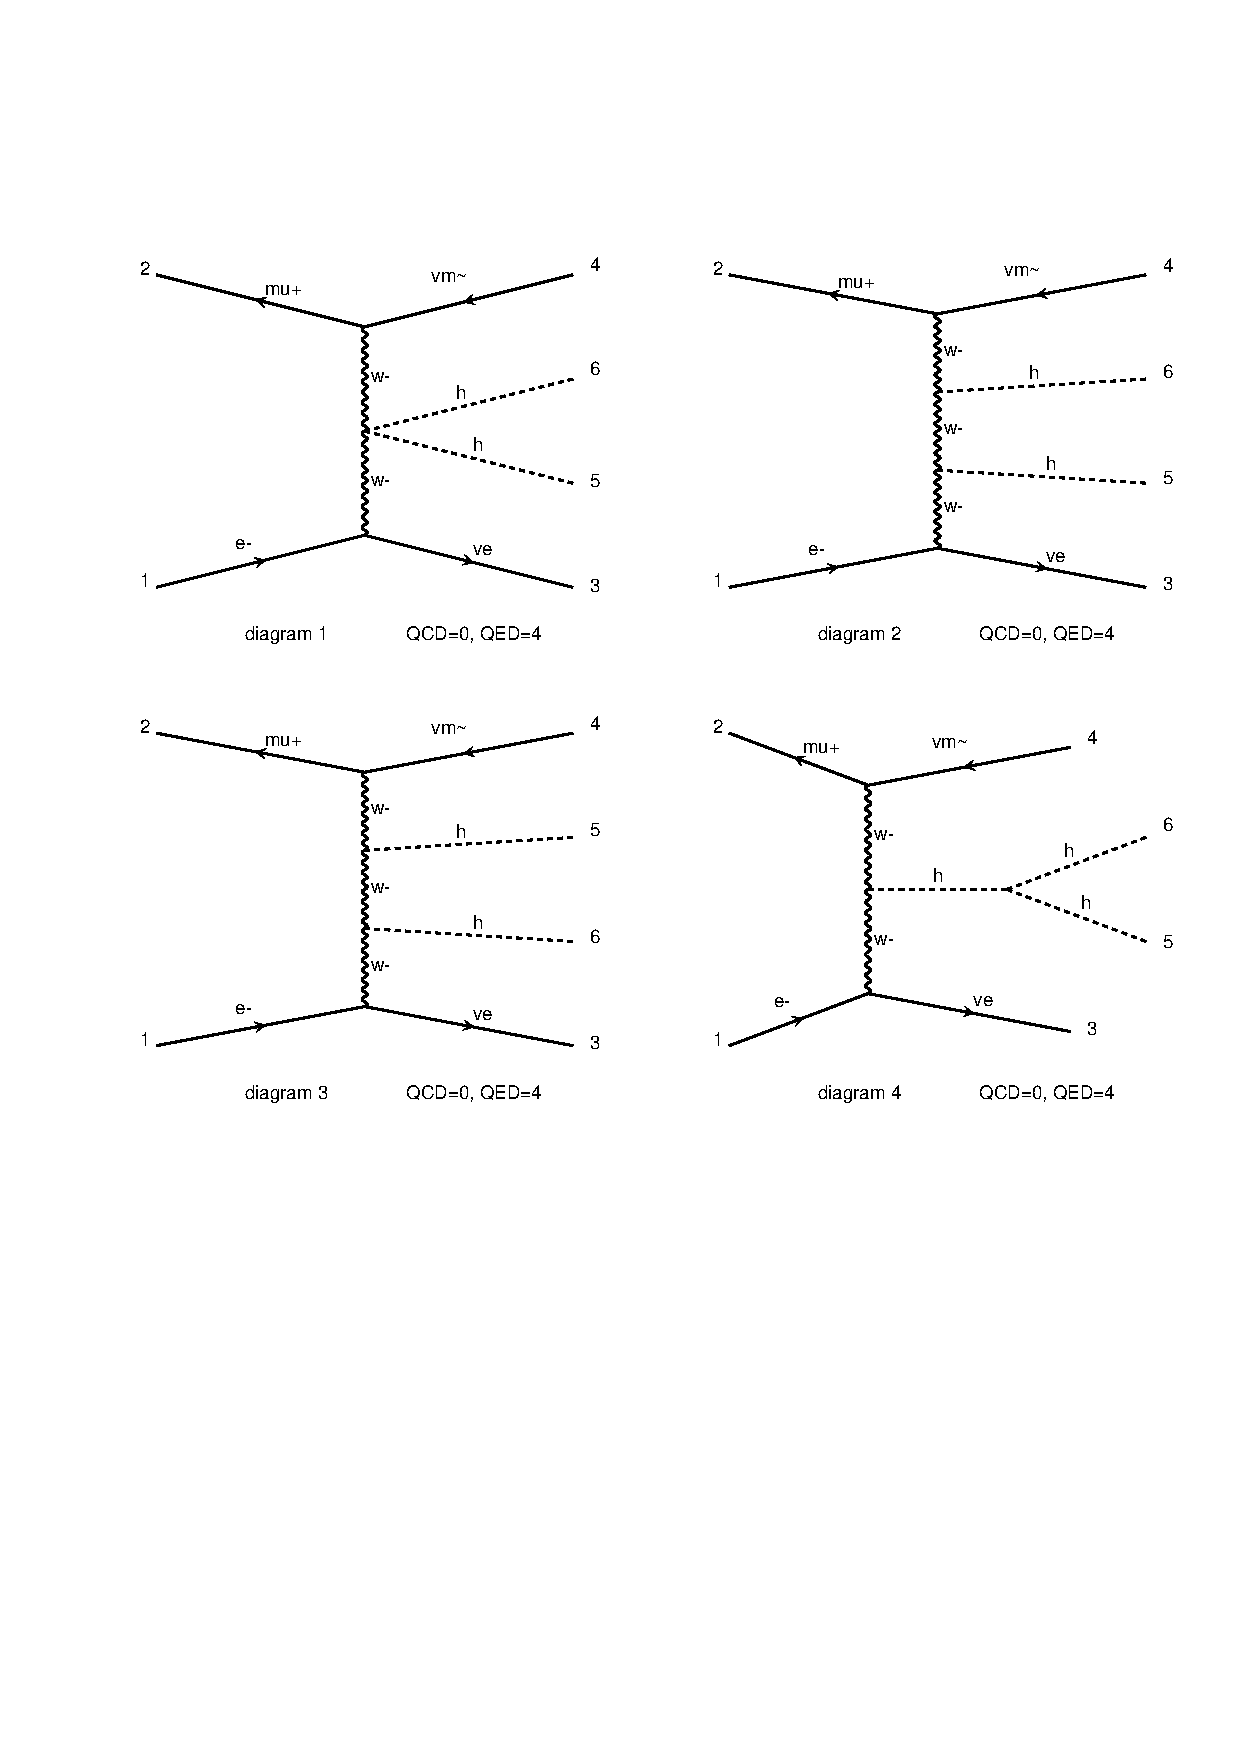
\includegraphics[width=\linewidth,height=0.42\textheight,keepaspectratio]{figures/CC_HH_diagrams_cropped.pdf}\caption{CC $e^-\mu^+\to\nu_e\bar\nu_\mu hh$.}\end{subfigure}\hfill
\begin{subfigure}[t]{0.48\linewidth}\centering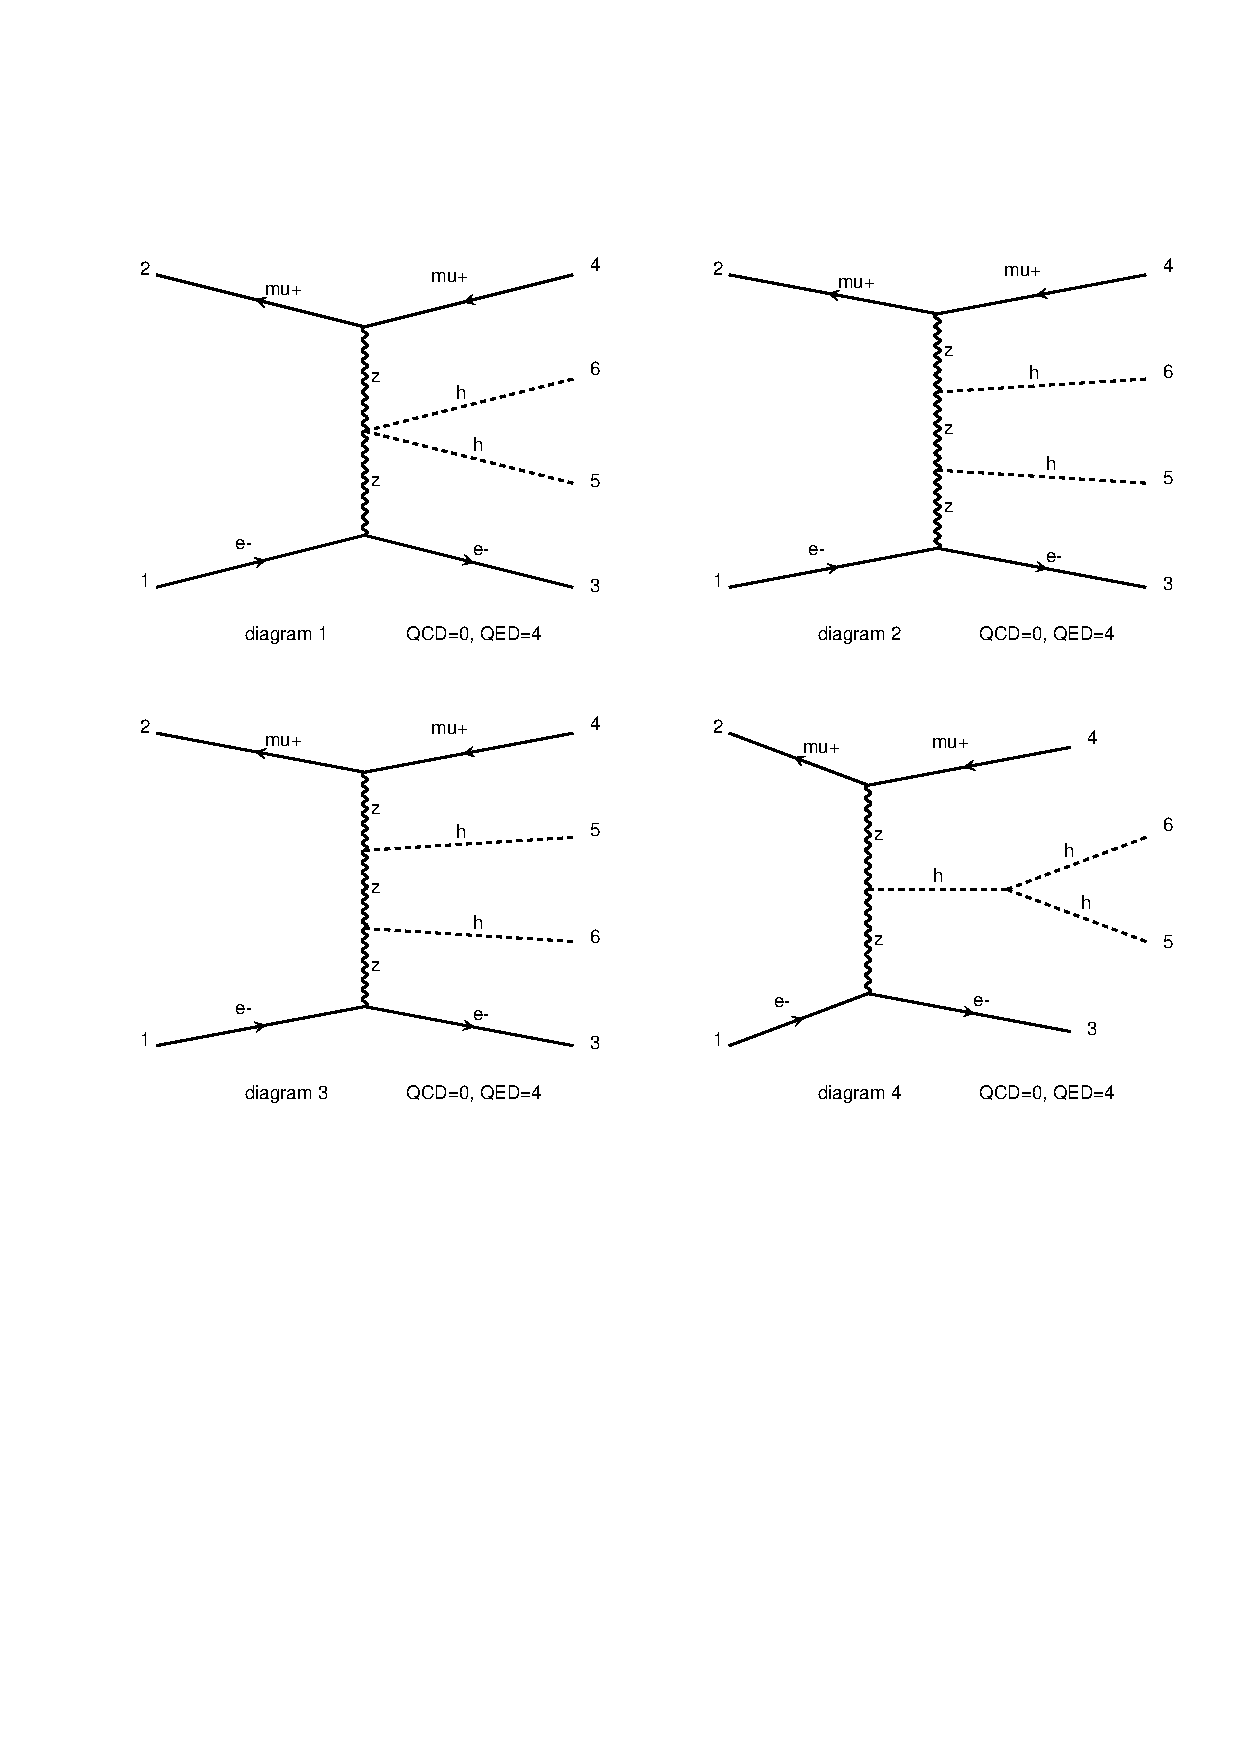
\includegraphics[width=\linewidth,height=0.42\textheight,keepaspectratio]{figures/NC_HH_diagrams_cropped.pdf}\caption{NC $e^-\mu^+\to e^-\mu^+hh$.}
\end{subfigure}
\caption{Genuine original MadGraph vector diagrams, preserved without substituting generic literature illustrations. The diagram IDs follow the source exports.}
\end{figure}


\textbf{Interpretation.} The full differential rate contains all squared and interference terms, for example $2\operatorname{Re}(\mathcal M_{h^*}\mathcal M_{hhVV}^*)$.\par Separately counting diagrams or omitting contact terms would not yield a universal, gauge-invariant extraction of a ``self-coupling contribution.'' The model must be varied consistently at the amplitude level. A next useful cross-check is to rerun selected reference points after varying $\kappa_3$ in a validated EFT/HEFT implementation and explicitly verify the anticipated polynomial dependence.




% PAGE 10
\newnote

\section{The 48-run CERN polarization campaign: reproducibility and results}
The completed campaign used MG5\_aMC v3.6.4 at LO with four processes, two \emph{exact} centre-of-mass energies and six positive-muon beam polarizations $P_{\mu^+}=0,20,40,60,80,100\%$. The electron was beam 1 and unpolarized, and the antimuon beam 2. Higgs particles were stable and no generation-level phase-space cuts were imposed. Each of the $4\times2\times6=48$ jobs requested/generated 30,000 events. All original result records were recovered; the package labels them \texttt{COMPLETED\_UNVALIDATED} because independent physics tests are not yet complete.

\begin{table}[H]
\centering\small
\caption{Selected inclusive cross sections (fb). Values are from the machine-readable source CSV; the uncertainties are generator Monte Carlo integration errors only.}
\begin{tabular}{@{}llrrr@{}}\toprule
$\sqrt{s}$ & Channel & $P=0\%$ & $P=80\%$ & $P=100\%$\\\midrule
1 TeV & CC $h$ & 210.540 & 378.570 & 421.150\\
 & CC $hh$ & 0.074384 & 0.133230 & 0.148239\\
 & NC $h$ & 20.835 & 24.476 & 25.402\\
 & NC $hh$ & 0.009620 & 0.011308 & 0.011723\\\midrule
2 TeV & CC $h$ & 386.010 & 695.000 & 772.690\\
 & CC $hh$ & 0.418510 & 0.754495 & 0.839521\\
 & NC $h$ & 38.991 & 45.829 & 47.642\\
 & NC $hh$ & 0.054712 & 0.064299 & 0.066770\\\bottomrule
\end{tabular}
\end{table}


The complete 48-row CSV with exact values, integration errors, generator seeds, job identifiers and event numbers accompanies this manuscript. To illustrate source precision rather than imply experimental accuracy, $\sigma(\CC hh,2\,\mathrm{TeV},80\%)=0.754495\pm0.001277$ fb. The quoted uncertainty is generated by the integration algorithm; it excludes uncertainty from missing higher orders, model parameters, collinear/forward treatment, detector response and machine conditions.

A rigorous reproducibility programme should repeat representative points with new independent seeds, compare numerical integration settings, verify electroweak parameter cards, and test NC lepton fiducial cut dependence. These tests are not replaced by the successful completion of 48 batch jobs. The original run cards and logs provide a useful baseline for them.





% PAGE 11
\newnote

\section{Polarization fits, cross-section ratios, and diagnostic plots}


For each process and energy the reported analysis fits the cross section as $\sigma(p)=a(1+Ap)$, where $p=P_{\mu^+}/100$. The inferred slopes are obtained from the absolute cross sections, avoiding treatment of multiple ratios with a common random denominator as independent observations.
\begin{table}[H]\centering\small
\caption{Numerical-fit polarization slopes $A$. These are fit/integration errors, not collider measurements.}
\begin{tabular}{@{}lcc@{}}\toprule Channel & 1 TeV & 2 TeV\\\midrule
CC $h$ & $0.9982\pm0.0020$ & $1.0007\pm0.0018$\\
CC $hh$ & $0.9934\pm0.0040$ & $1.0053\pm0.0039$\\
NC $h$ & $0.2181\pm0.0012$ & $0.2208\pm0.0011$\\
NC $hh$ & $0.2186\pm0.0022$ & $0.2204\pm0.0022$\\\bottomrule
\end{tabular}\end{table}
\begin{figure}[H]\centering
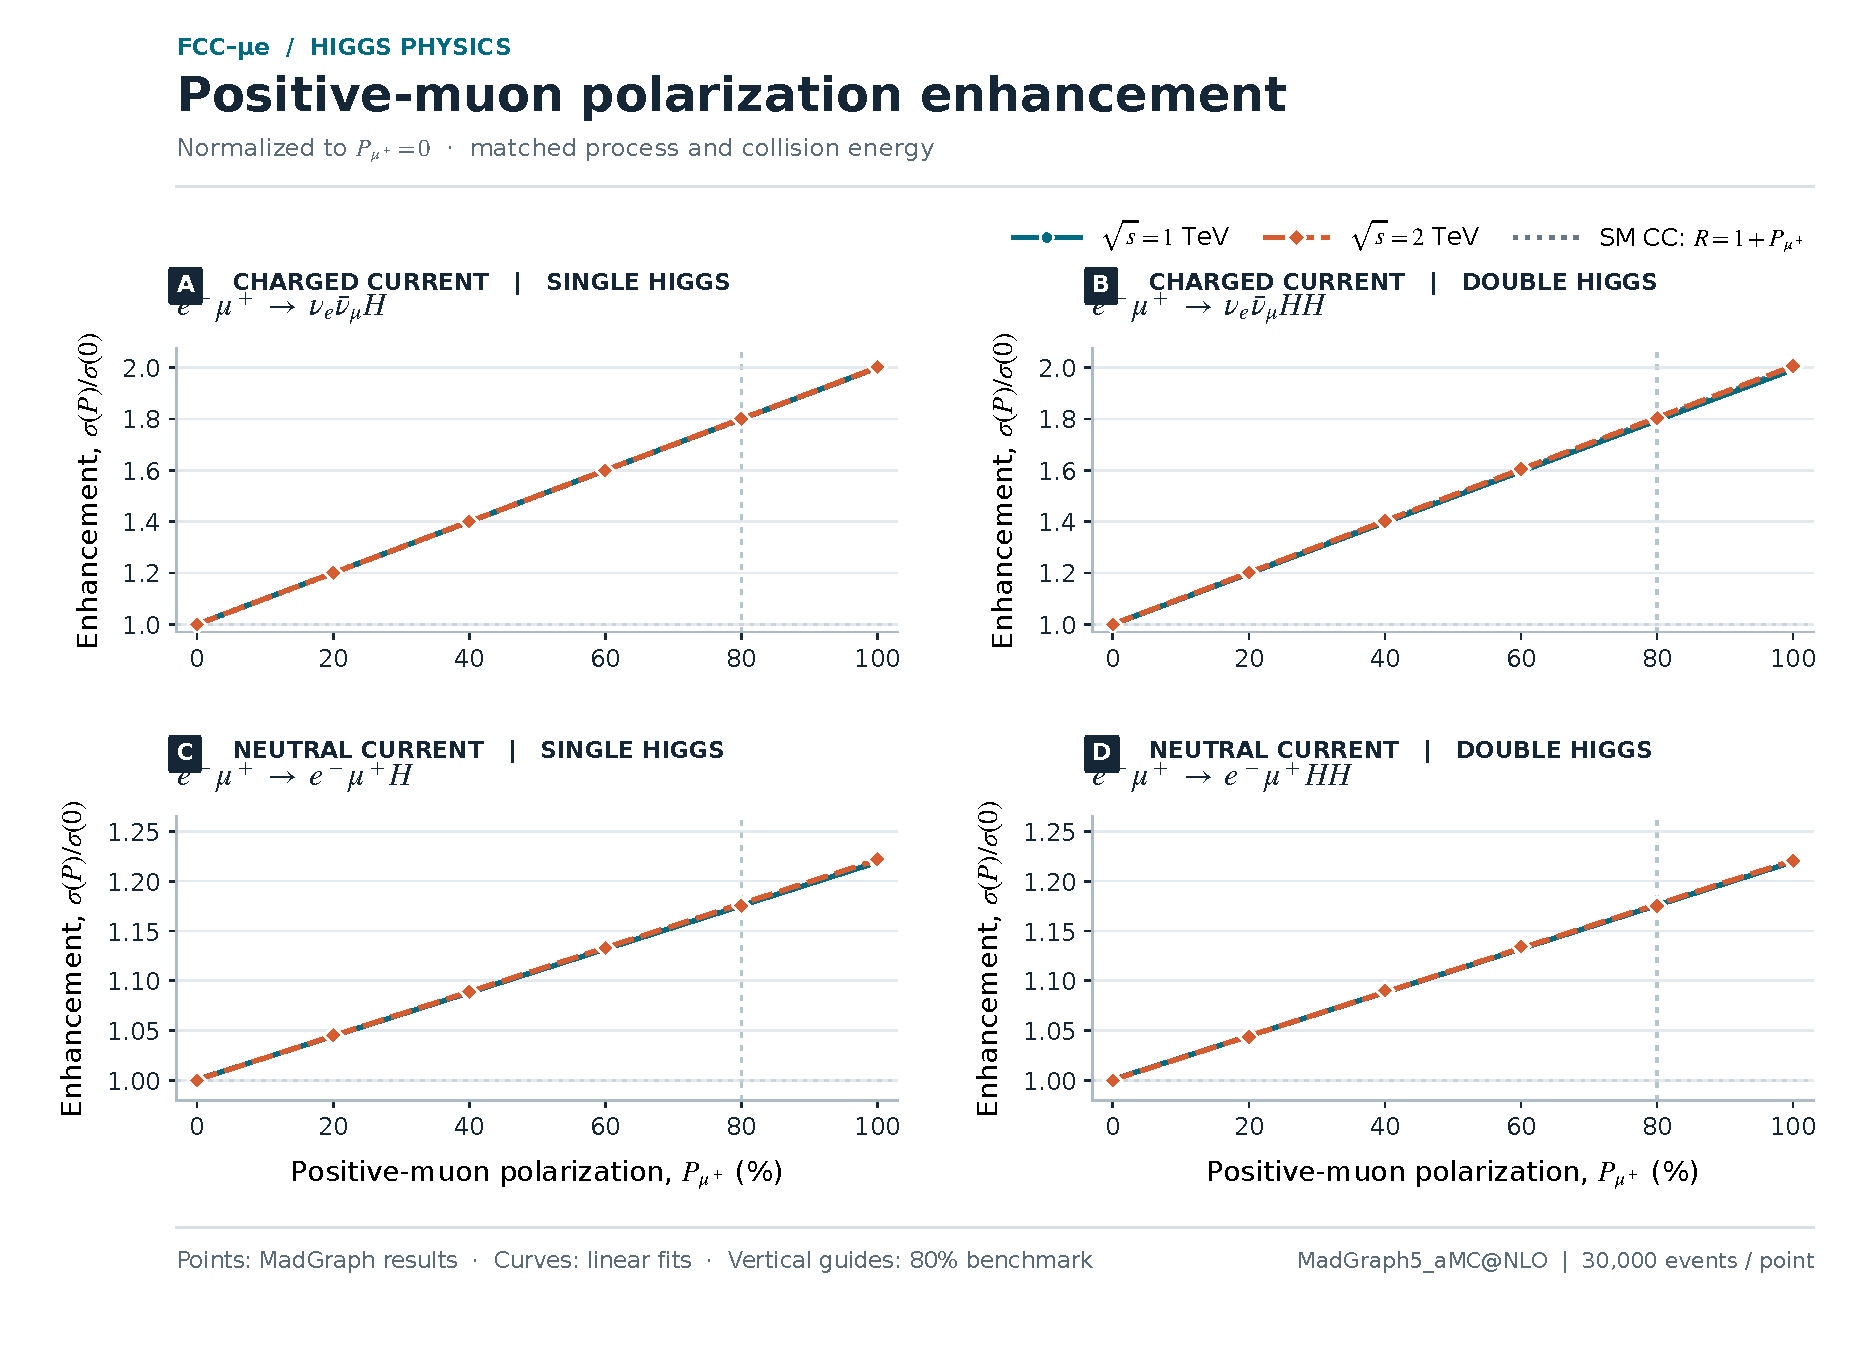
\includegraphics[width=0.97\linewidth,height=0.33\textheight,keepaspectratio]{figures/Figure_2_polarization_ratios.pdf}
\caption{Ratios $\sigma(P)/\sigma(0)$ in the four inclusive channels, from the original 48 CERN runs. The CC slope is near 1, whereas the NC slope is near 0.22. Error bars reflect numerical integration.}
\end{figure}

The separation of CC and NC slopes is the cleanest physical finding: for $+80\%$ antimuon polarization, the CC rate enhancement is close to 1.8, while the NC enhancement is about 1.175. The relative growth from exact 1 to 2 TeV is $1.833$ for CC $h$, $1.871$ for NC $h$, $5.626$ for CC $hh$, and $5.687$ for NC $hh$ at $P=0$. The close similarity of the NC $h$ and $hh$ slopes indicates that the dominant helicity dependence arises in the initial $Z$-current factors. It is not, by itself, a determination of the weak mixing angle: luminosity, polarization calibration, coupling correlations and realistic fiducial phase space remain indispensable.



% PAGE 12
\newnote

\section{Charged-current $hh\to4b$: resonant and complete final states}
An earlier CERN programme investigated $e^-\mu^+\to\nu_e\bar\nu_\mu hh\to\nu_e\bar\nu_\mu b\bar b b\bar b$ and the corresponding complete $e^-\mu^+\to\nu_e\bar\nu_\mu b\bar b b\bar b$ final state. Parallel comparisons were made with symmetric $\mu^+\mu^-$ collisions. These older results are \emph{fiducial parton-level} calculations; they must not be equated with the later stable-Higgs inclusive rates.

The selection requires four bottom/antibottom partons satisfying $|\eta_b|<5$ and two distinct opposite-charge $b\bar b$ combinations each within $110<m_{b\bar b}<130$ GeV, without a minimum bottom-parton $p_T$ cut. This is a generator-level pairing/selection, not realistic jet clustering, bottom tagging or detector Higgs reconstruction. The actual pairing algorithm and any neutrino-flavour sums should be treated as part of the source run-card definition.


\begin{table}[H]
\centering\small
\caption{Selected historical fiducial cross sections [fb]. Entries are $P_{\mu^+}=0\%/80\%$ for the studied configurations.}
\begin{tabular}{@{}llcc@{}}\toprule Collider & $\sqrt{s}$ & Resonant $hh\to4b$ & Complete $\nu\bar\nu4b$\\\midrule
FCC-$\mu e$ & 0.980 TeV & 0.04912 / 0.08816 & 0.05355 / 0.09195\\
$\mu^+\mu^-$ & 1.000 TeV & 0.07047 / 0.11582 & 0.07530 / 0.12472\\
FCC-$\mu e$ & 1.913 TeV & 0.26478 / 0.47611 & 0.28157 / 0.50745\\
$\mu^+\mu^-$ & 2.000 TeV & 0.30624 / 0.54606 & 0.32480 / 0.57873\\\bottomrule
\end{tabular}\end{table}


The complete final-state amplitude includes resonant, singly resonant, nonresonant and interference pieces. It is therefore invalid to identify the ``background'' as the complete 4b cross section minus the resonant $hh$ sample without a consistent amplitude-level and event-definition analysis. Double counting is also possible if independently generated $hh$, $b\bar b h$ and complete 4b samples are naively added.

A critical numerical caveat is that the earlier model card used $\mathrm{BR}(h\to b\bar b)=0.844640$, whereas a conventional 125-GeV SM prediction is approximately 0.582 \cite{pdg}. The resonant double-decay probability is affected quadratically. One must harmonize branching ratios or regenerate samples before projecting experimental yields; a simple rescaling is not generally appropriate for the complete interfering amplitude.





% PAGE 13
\newnote

\section{NC four-bottom channels, associated $b\bar b h$, and muon $Zh$}
The neutral-current historical portfolio studied $e^-\mu^+\to e^-\mu^+hh\to e^-\mu^+4b$, associated $e^-\mu^+\to e^-\mu^+b\bar b h\to e^-\mu^+4b$, the complete $e^-\mu^+4b$ amplitude, and a diagnostic sample excluding internal Higgs contributions. The earlier NC event generation imposed $p_{T,\ell}>1$ GeV on outgoing charged leptons in addition to the four-bottom angular and $110$--$130$ GeV pairing selections. Thus these are emphatically not the uncut inclusive NC rates shown on pp. 10--11.
\begin{table}[H]\centering\small
\caption{Preliminary NC fiducial cross sections at approximately 0.980 TeV, unpolarized.}
\begin{tabular}{@{}lr@{}}\toprule Channel & $\sigma_{\rm fid}$ [fb]\\\midrule
NC $hh\to4b$ & 0.006382\\
Associated $b\bar b h\to4b$ & 0.012925\\
Complete $e^-\mu^+4b$ & 0.007713\\
Higgs-excluded continuum diagnostic & 0.0008253\\\bottomrule
\end{tabular}\end{table}
The continuum estimate is limited by 88 accepted events among 50,000 generated. There is also a \emph{specific unresolved consistency problem}: the full-NC-4b rate is below the separately generated associated-$b\bar b h$ rate. One cannot conclude that interference alone explains this ordering, because process definitions, cuts, normalization and Monte Carlo convergence must first be reconciled. This mismatch is an actionable audit task, not an established interference measurement. Higher-energy associated-$b\bar b h$ examples ($\sim0.081843$ fb at FCC-$\mu e$ 1.913 TeV and $\sim0.094913$ fb at $\mu^+\mu^-$ 2 TeV, both at $+80\%$ in their reported configurations) remain preliminary pending cut-level verification.

A distinct benchmark is $\mu^+\mu^-\to Zh\to (b\bar b)(b\bar b)$: at 1 TeV the LO cross section before/after the selected cuts is $1.56450/1.52716$ fb, while at 2 TeV it is $0.37888/0.36929$ fb. These runs used $|\eta_b|<5$ and two assigned $b\bar b$ masses in the \emph{wider} $80$--$130$ GeV window, without a minimum bottom-parton $p_T$ cut. The flavour-diagonal $s$-channel annihilation contribution of $\mu^+\mu^-$ has no ordinary neutral-current $\mu^+e^-$ analogue. The final state is also distinct from neutrino-associated $hh\to\nu\bar\nu4b$.




% PAGE 14
\newnote

\section{From inclusive cross sections to observable event samples}


An inclusive LO production rate is only the first factor in a realistic sensitivity analysis. For a specified exclusive signal selection $i$, the expected event yield takes the schematic form
\begin{equation}\label{eq:yields}
N_i=\Lumi_{\rm int}\sum_{c}\sigma_c(\bm\kappa)\,
\mathrm{BR}_c(\bm\kappa)\,\eps_{c,i}(\bm\kappa,\bm\theta)+B_i(\bm\theta),
\end{equation}
where $c$ indexes physical signal/decay channels, $\eps$ includes fiducial acceptance and reconstruction, $\bm\theta$ denotes nuisance parameters and $B_i$ is background. The production coupling and Higgs decay parameters may be correlated, so a consistent width/branching-ratio treatment is required.

As an explicitly \emph{illustrative}, not established FCC-$\mu e$ luminosity assumption, take $\Lumi_{\rm int}=3\,\mathrm{ab}^{-1}$ and $P_{\mu^+}=+80\%$. The reported inclusive CC $hh$ rates imply $N_{hh}\approx400$ produced pairs at 1 TeV and $\approx2263$ at 2 TeV before Higgs decays and acceptance; the corresponding NC yields are about 34 and 193. If both Higgs bosons decay to $b\bar b$ with a representative SM branching fraction 0.582, the raw $4b$ fraction is $(0.582)^2\simeq0.339$. A naive four-tag factor $\eps_b^4$, e.g. $(0.7)^4\simeq0.24$, would reduce this further, even before kinematic cuts, jet pairing, showering, backgrounds and beam-induced effects. None of these illustrative factors can be taken as a detector-level efficiency estimate.

Potential discriminants include reconstructed $m_{hh}$, two $m_{b\bar b}$ peaks, angular separation of $b$ jets, total visible energy, missing transverse momentum and NC final-state charged-lepton tags. The correct background model must incorporate genuine irreducible final-state amplitudes, reducible heavy flavour and mistags where relevant, as well as detector/beam-induced background overlays. The energy-asymmetric machine changes object rapidities, particularly the outgoing charged leptons in NC events. Finally, the running programme must specify whether a given polarization setting retains the same delivered luminosity: a factor 1.8 in CC cross section does not automatically yield a factor 1.8 improvement in precision.




% PAGE 15
\newnote

\section{A Higgs-coupling measurement programme: parameters and theory control}
A quantitative study should begin with a declared parameter basis. In a phenomenological HEFT-like normalization, choose the set $\{\kappa_W,\kappa_Z,\kappa_{2W},\kappa_{2Z},\kappa_3\}$; the quartic $\kappa_4$ can be introduced when assessing triple Higgs. The single-H CC and NC samples help constrain the two $hVV$ factors, while $hh$ rates and shapes add information about $hhVV$ and $\lambda_3$. If the target is a one-parameter $\kappa_3$ projection, it must explicitly say that the other couplings are fixed to their SM values; otherwise the inferred constraint is generally not robust.

A useful fit sequence is: (i) fit single-H production and branching information to control $\kappa_W,\kappa_Z$ and normalization nuisances; (ii) evaluate $hh$ coefficient templates at several physically consistent anomalous-coupling points; (iii) combine total and differential yields at both energies and beam polarizations; and (iv) profile over nuisance parameters and correlated gauge-Higgs variations. The rate-only $\sigma_{hh}(\kappa_3)$ is a quadratic polynomial at fixed other couplings, but a multidimensional fit can have richer interference structure and degenerate contours. No coupling limits have been produced by the current 48-run SM scan.

In a linear gauge-invariant SMEFT, the scalar doublet transforms under $SU(2)_L\times U(1)_Y$ and effective operators correlate the modifications of $hVV$, $hhVV$, fermionic currents and other amplitudes. A HEFT parameterization treats the physical scalar more flexibly and may allow distinct coefficients $a$ and $b$ in the Goldstone sector. Both are useful, but they answer different questions. An EFT study must specify operator normalization, input-parameter scheme, truncation order (linear versus quadratic in Wilson coefficients), renormalization scale if relevant, and the domain of validity $E<\Lambda$ of the expansion.

One physically motivated separation uses $\kappa_3$ to modify the off-shell scalar-mediated part and $\kappa_{2V}$ to modify the two-Higgs gauge contact. Yet those apparent ``directions'' are not automatically independent parameters of a given gauge-invariant SMEFT truncation. For first exploratory grids they may be treated within a validated HEFT model; a complementary SMEFT interpretation can then translate observable patterns into operator coefficients subject to matching and unitarity constraints. Existing detector-level electron--muon $hhWW$ phenomenology must be cited as prior art, notably Cao \emph{et al.} \cite{cao}. The new contribution should be a coherent combined CC/NC, polarization and shape analysis with realistic machine assumptions.




% PAGE 16
\newnote

\section{Differential observables and interference-based discrimination}
A total $hh$ cross section compresses potentially useful kinematic information. The most direct differential variable is $m_{hh}=\sqrt{(p_{h_1}+p_{h_2})^2}$, which samples the virtual-Higgs propagator and the high-energy contact/gauge exchange contributions differently. Further observables include $p_{T,h}$, the $hh$ system transverse momentum and rapidity, the opening angle between Higgs bosons, and the momentum transfers to outgoing leptons in NC events. In CC events, missing transverse momentum and the distribution of visible Higgs decay products help select the weak-fusion topology.

\begin{figure}[H]\centering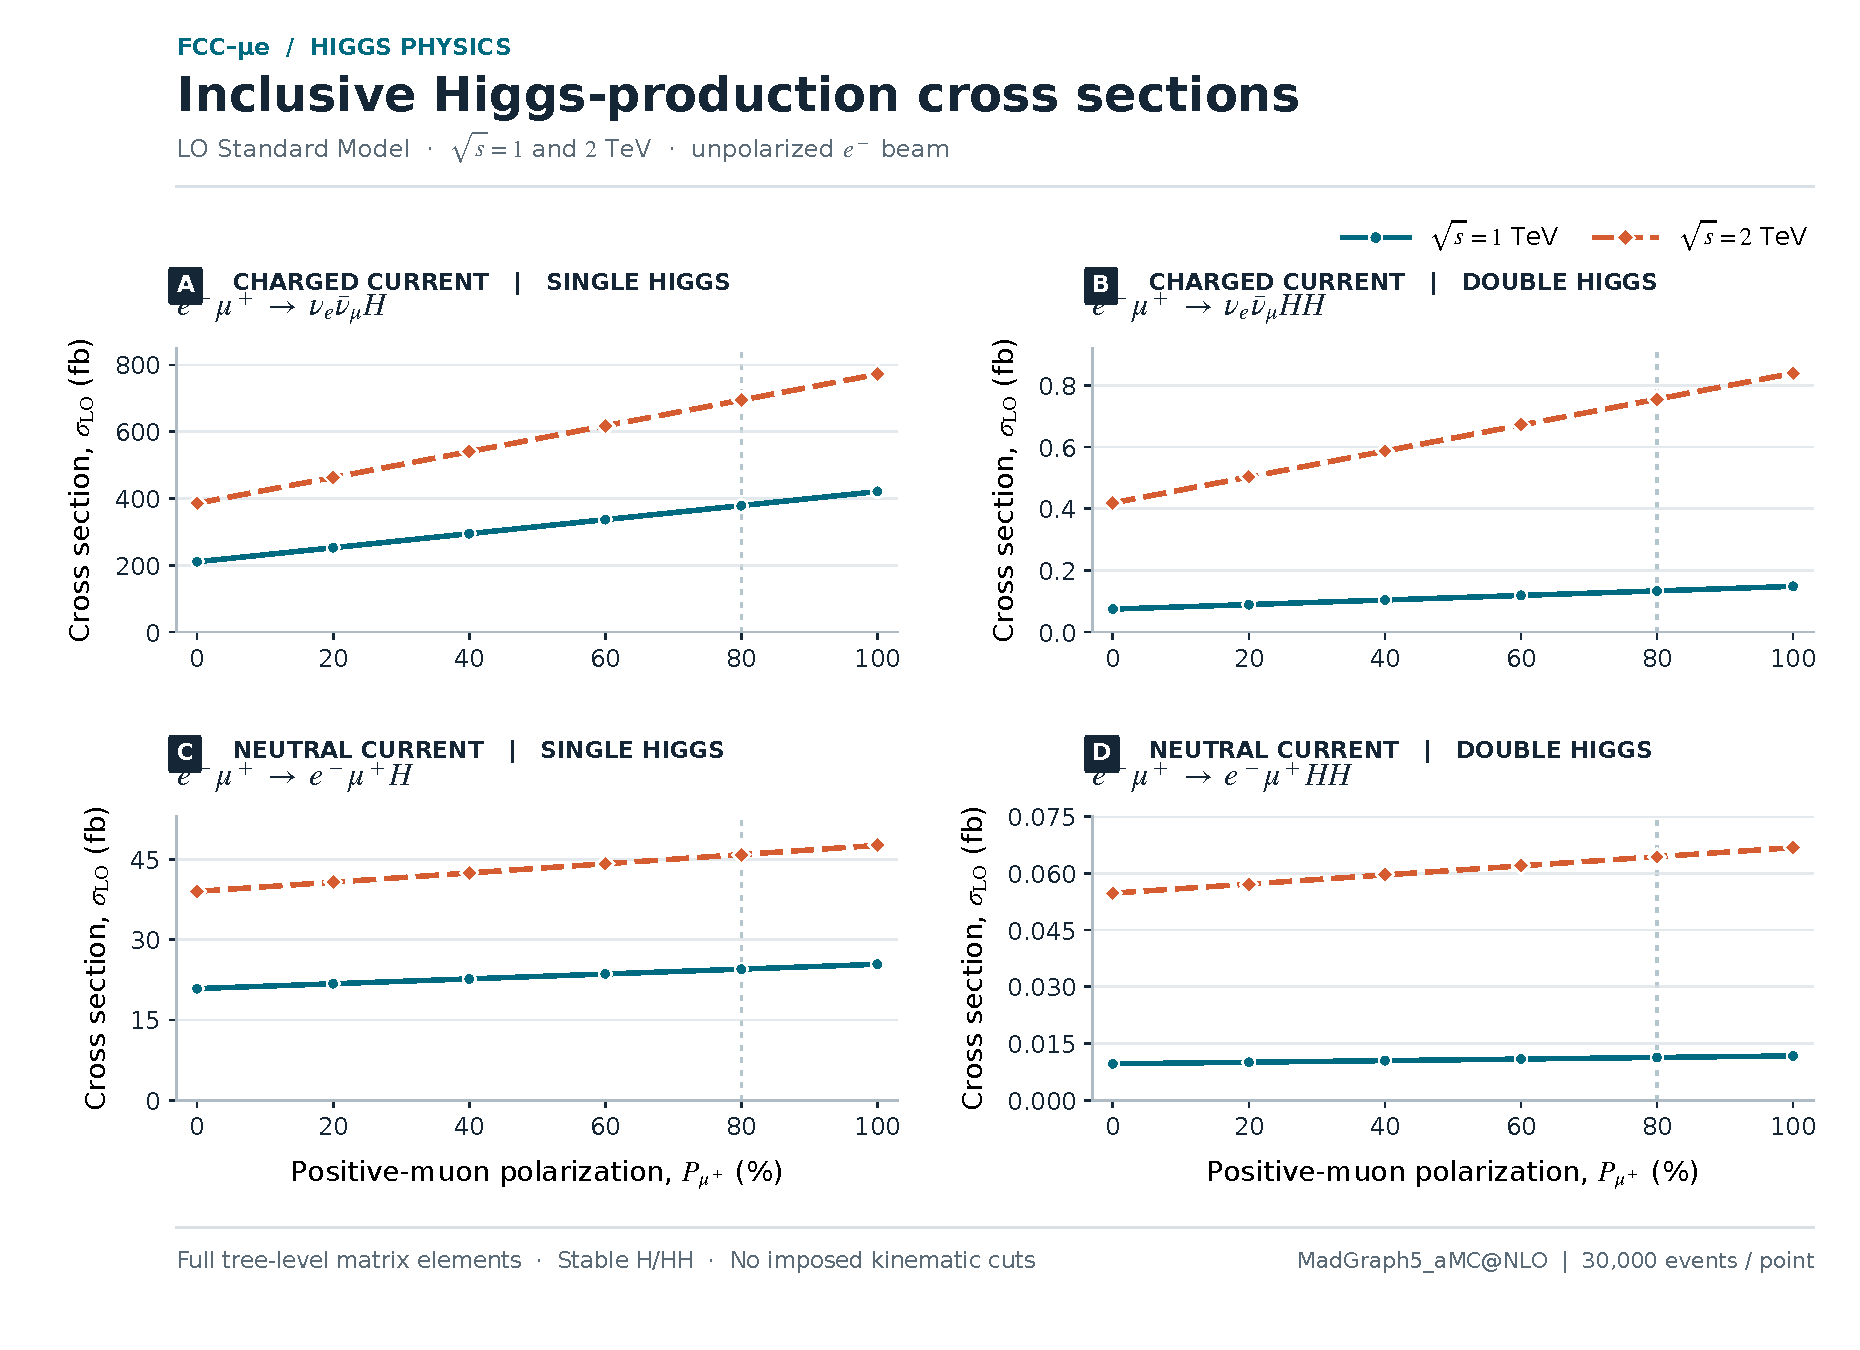
\includegraphics[width=0.97\linewidth,height=0.34\textheight,keepaspectratio]{figures/Figure_1_absolute_cross_sections.pdf}
\caption{Source-derived LO single- and double-Higgs inclusive cross sections at exact 1 and 2 TeV versus the six positive-muon polarization points. The figure is a baseline for future \emph{differential} anomalous-coupling studies, not an anomalous-coupling prediction.}
\end{figure}
The high-$m_{hh}$ tail may be sensitive to anomalous $hhVV$ interactions when the Standard Model high-energy cancellations are modified. Near threshold, the relative influence of the trilinear scalar exchange can be larger. Both observations depend on selections: a highly boosted configuration or tight visible acceptance can sculpt the distributions, and a power-enhanced EFT contribution at large momentum transfer may approach the validity limit of the EFT itself. Thus the final fit must compare finite detector-level bins, not extrapolate an unregulated partonic tail into an arbitrarily high-energy region.

For reliable numerical templates, use common electroweak inputs and process cuts across all coupling points, independent seeds for selected spot checks, and explicit event-sample overlap rules for resonant and complete amplitudes. Retain full systematic covariance or nuisance parameter effects rather than turning each bin's Monte Carlo integration error into an experimental uncertainty. A source-controlled analysis should archive both the generator parameters and a compact histogram production code.




% PAGE 17
\newnote

\section{From cross sections to likelihoods and projected sensitivity}
A genuine measurement projection needs a statistical model and backgrounds. For observed counts $n_i$ in bins of $m_{hh}$, lepton kinematics and event categories, define the expected bin content
\begin{equation}
\mu_i(\bm\kappa,\bm\theta)=\Lumi_{\rm int}
 \sum_c\sigma_{c,i}(\bm\kappa)\,
 \mathrm{BR}_c(\bm\kappa)\,\eps_{c,i}(\bm\theta)
 +b_i(\bm\theta),
\end{equation}
where $\bm\theta$ describes integrated luminosity, antimuon polarization calibration, tagging efficiency, acceptance, background normalization/shape and theory effects. A standard binned likelihood is
\begin{equation}\label{eq:likelihood}
\mathcal L(\bm\kappa,\bm\theta)
=\prod_i\frac{\mu_i^{n_i}e^{-\mu_i}}{n_i!}
\prod_a\pi_a(\theta_a),\qquad
q(\bm\kappa)=-2\ln\frac{\mathcal L(\bm\kappa,\hat{\bm\theta}_{\bm\kappa})}
{\mathcal L(\hat{\bm\kappa},\hat{\bm\theta})}.
\end{equation}
The profile construction makes the underlying uncertainty assumptions explicit. Asimov datasets can be used for expected constraints only \emph{after} signals, backgrounds and nuisance models are specified. For Poisson bins with known background the expected information scales schematically as $I_{ab}=\sum_i(\partial_a\mu_i)(\partial_b\mu_i)/\mu_i$; the matrix can be singular if two coupling directions yield nearly identical spectra. This motivates complementary CC and NC processes, multiple energies and beam-polarization settings.

A minimal baseline sensitivity scenario should record: actual feasible luminosity for each beam configuration, Higgs branching-ratio correlations with $\bm\kappa$, fiducial acceptances from detector simulation, main irreducible and reducible backgrounds, treatment of forward electrons and antimuons, and higher-order electroweak uncertainties. A ``statistical only'' scenario may be included for transparency but must be visibly distinct from a robust experimental projection. Likewise a literature estimate quoted in the FCC-$\mu e$ proposal is a tentative rescaling of muon-collider expectations, not a measured or directly calculated $\kappa_3$ limit from the present work.

The concrete output of the next phase should be likelihood-ready binned templates and their provenance, not merely another table of inclusive SM cross sections. A blinded internal validation should first reproduce the known SM rates and the analytic CC polarization dependence, then check closure tests on injected nonstandard coupling points.




% PAGE 18
\newnote

\section{Triple Higgs and the quartic self-coupling: a feasibility test}
A forward extension is charged-current $e^-\mu^+\to\nu_e\bar\nu_\mu hhh$ and neutral-current $e^-\mu^+\to e^-\mu^+hhh$, whose proposed unrestricted SM MadGraph commands are
\begin{center}\ttfamily\small
 generate e- mu+ > ve vm\textasciitilde{} h h h QCD=0\\
 generate e- mu+ > e- mu+ h h h QCD=0
\end{center}
The $VV\to hhh$ amplitudes can involve the quartic self-coupling $\lambda_4$, one or more trilinear $\lambda_3$ insertions and gauge-Higgs contact/propagation contributions. Consequently, $hhh$ could, in principle, complement $hh$ by accessing a qualitatively new combination of Higgs-potential parameters. It is not a clean isolated measurement of $\kappa_4$: other couplings and interference remain essential.

The minimum on-shell invariant mass is $m_{hhh}\ge3m_h\simeq375$ GeV. At exact 1 and 2 TeV the initial lepton CM energy is above threshold, but the virtual weak bosons carry only a fraction of that energy and phase space is restricted. Small SM rates, limited polarization-specific luminosity, complicated multibody final states and beam/detector backgrounds may make the measurement unfeasible. No numerical $hhh$ cross section has yet been computed in this project, and no quartic-coupling sensitivity should be invented.

A sensible initial campaign computes CC and NC SM rates at 1 and 2 TeV for $P_{\mu^+}=0,80,100\%$, with stable Higgs bosons and independently audited integration. The expected CC enhancement $\sim1+p$ provides a further cross-check. Only if numerically stable rates are appreciable should the study advance to decays and to a $\kappa_3$--$\kappa_4$ scan. For a transparent \emph{illustrative} integrated luminosity $3\,{\rm ab}^{-1}$, ten produced inclusive events would require $\sigma\ge10/(3000\,{\rm fb}^{-1})=0.00333$ fb. The all-bottom decay fraction under the representative SM $h\to b\bar b$ value 0.582 is approximately $0.582^3\simeq0.197$ before six-tag inefficiency; $4b2\tau$ or $4b2\gamma$ may improve background discrimination despite smaller branching ratios.

The decision criterion is physics feasibility: reliable SM event yield, theoretical sensitivity shape, reconstruction strategy and realistic background expectation. A null or tiny expected $hhh$ yield is itself useful for redirecting the research towards $hh$ or higher-energy exploratory scenarios.




% PAGE 19
\newnote

\section{A joint research roadmap and validation gates}
The completed results suggest an ordered collaboration programme rather than independent, unrelated generator exercises. The first deliverable is a controlled Standard Model reference: agree on model version and electroweak scheme, Higgs branching fractions, beam energies, polarization signs, cuts and numerical settings, and then rerun representative CC and NC $h/hh$ points with independent seeds. The forward NC region requires an explicit lepton-angle/$p_T$ stability study. The historical four-bottom samples must be regenerated or coherently renormalized, and the NC complete-four-bottom versus associated-$b\bar b h$ discrepancy must be resolved at identical phase-space definitions.

\begin{table}[H]\centering\small\caption{Proposed work packages; individual assignments should be agreed at the meeting, not presumed here.}
\begin{tabularx}{\linewidth}{@{}p{0.13\linewidth}X p{0.27\linewidth}@{}}\toprule
Stage & Scientific task & Testable deliverable\\\midrule
I & Common SM cards, seeds, diagram/full-amplitude QA; NC forward tests; historical BR and sample reconciliation & Verified baseline archive and cross-section comparison\\
II & Gauge-consistent $\kappa_3$--$\kappa_{2W,2Z}$ grids, 1/2 TeV and polarization variants & Validated matrix-element templates and distributions\\
III & Showering, jet and lepton acceptance, $4b$ backgrounds, detector scenarios & Fiducial response matrices and background model\\
IV & Binned multi-channel likelihood with FCC-ee priors where justified & Qualified projected coupling sensitivity and degeneracy maps\\
V & SM $hhh$ feasibility and possible $\kappa_4$ extension & Feasibility memo with honest yield/background thresholds\\\bottomrule
\end{tabularx}\end{table}
The distinctive paper-level question is whether \emph{combined polarized CC and NC Higgs-pair production, calibrated by single Higgs and differential observables}, can disentangle Higgs self-interactions from gauge-Higgs contact modifications. This goes beyond showing energy-growing SM cross sections. Existing lepton-collider $hhWW$ analyses, including the 2024 study by Cao, Cheng, Liu and Wang \cite{cao}, already provide a baseline of prior phenomenology. A novel claim must be supported by improved process complementarity, a realistic polarization/luminosity scenario or a genuinely multidimensional inference.

For the first collaboration meeting, decisions should include: the official machine working points and realistic polarized luminosities; choice of EFT/HEFT model and operator basis; ranking CC/NC channels for detector work; common branching-ratio and decay treatment; reproducibility checks and code/data ownership; and concrete milestones for the first shared phenomenology note. These decisions should be explicitly recorded before a paper sensitivity plot is generated.




% PAGE 20
\newnote


\section{Conclusions and scientific references}
The CERN calculations establish an internally consistent preliminary LO baseline for $\mu^+e^-$ Higgs physics: CC $h$ and $hh$ rates are generally greater than corresponding NC rates; the normalized antimuon polarization enhancement is near $1+p$ for CC and around $1+0.22p$ for NC; and $hh$ production rises much faster than single-H production between exact 1 and 2 TeV. Original full-process MadGraph diagrams demonstrate that the trilinear scalar exchange, separate Higgs-emission graphs and $hhVV$ contact graphs are included together with interference. Earlier four-bottom and muon-collider associated-$Zh$ calculations extend the phenomenological context but have distinct phase-space cuts, branching-ratio inputs and normalization limitations.

The physics programme now must progress from SM benchmarks to consistently parametrized $\kappa_3$--$\kappa_{2V}$ grids, differential $m_{hh}$ information, validated event and detector selections, and likelihood fits including luminosity and polarization constraints. Triple-Higgs is worth a tightly scoped feasibility test, not an unsupported $\kappa_4$ precision claim. The first indispensable tasks remain the independent-seed and forward-region checks and reconciliation of the older four-bottom samples. These define a scientifically defensible path from a successful computing campaign to a credible collaborative Higgs-coupling analysis.

\vspace{2pt}\noindent\textbf{Selected references and primary input sources}
\begin{thebibliography}{9}\setlength{\itemsep}{1pt}\small
\bibitem{piotr} K.~Piotrzkowski, ``FCC-$\mu e$: High Energy, High Luminosity Muon-Electron Collider \& Neutrino Factory at CERN,'' \href{https://arxiv.org/abs/2610.40451}{arXiv:2610.40451v2} (revised 5 Nov. 2026), especially Table 1 and Sections 1--4.
\bibitem{fcc} FCC Collaboration, ``Future Circular Collider Feasibility Study Report, Vol.~1: Physics, Experiments, Detectors,'' \emph{Eur. Phys. J. C} \textbf{85}, 1468 (2025); \href{https://doi.org/10.1140/epjc/s10052-025-15077-x}{doi:10.1140/epjc/s10052-025-15077-x}; note the 2026 erratum.
\bibitem{cao} Q.-H.~Cao, K.~Cheng, Y.~Liu and X.-R.~Wang, ``Measuring $hhWW$ coupling at lepton colliders,'' \emph{Phys. Rev. D} \textbf{109}, 073005 (2024); \href{https://doi.org/10.1103/PhysRevD.109.073005}{doi:10.1103/PhysRevD.109.073005}.
\bibitem{pdg} Particle Data Group, ``Status of Higgs Boson Physics,'' \emph{Review of Particle Physics} (2024), Table 11.3, \href{https://pdgweb.lbl.gov/2024/reviews/rpp2024-rev-higgs-boson.pdf}{review PDF}.
\bibitem{mg5} J.~Alwall \emph{et al.}, ``The automated computation of tree-level and next-to-leading order differential cross sections, and their matching to parton shower simulations,'' \emph{JHEP} \textbf{07} (2014) 079, \href{https://doi.org/10.1007/JHEP07(2014)079}{doi:10.1007/JHEP07(2014)079}.
\bibitem{int48} H.~Khanpour and collaborators, ``FCC-$\mu e$ inclusive Higgs polarization scan: 48 MadGraph runs, original cards, cross-section CSV and audited figures,'' preliminary internal CERN calculation archive (Nov. 2026), bundled data files.
\bibitem{int4b} H.~Khanpour and collaborators, ``FCC-$\mu e$/$\mu\mu$ $hh\to4b$, full $4b$, associated-$b\bar bh$ and $Zh$ cross-section checks,'' preliminary internal CERN reports (Oct. 2026), provenance described in source manifest.
\end{thebibliography}

\vfill
\noindent{\color{aghgreen}\rule{\linewidth}{1pt}}\\[-2pt]
{\footnotesize\color{gray}Internal scientific discussion draft. The numerical integration errors reported herein are not experimental, detector or full theory uncertainties.}



\end{document}


